\documentclass[11pt,a4paper,twoside,openright]{book}

\documentclass{standalone}

\usepackage{fontspec}
\usepackage{unicode-math}

\setmainfont{QTBrushStroke}
%\setsansfont{CMU Sans Serif}
%\setmonofont{CMU Typewriter Text}


\usepackage{tikz}
\usepackage{circuitikz}
\usetikzlibrary{shadings}
\usepackage{graphicx}

\usepackage{xcolor}

\definecolor{Fortran}{HTML}{734F96}

\newcommand{\lts}{20pt}
\newcommand{\chisize}{60pt}
\newcommand{\fpc}{1.0}


\hypersetup{
    bookmarks=true, 		% show bookmarks bar?
    unicode=true,  		% non-Latin characters in Acrobat’s bookmarks
    pdftoolbar=true,        % show Acrobat’s toolbar?
    pdfmenubar=true,        % show Acrobat’s menu?
    pdffitwindow=true,      % page fit to window when opened
    pdftitle={Electrochemistry},    % title
    pdfauthor={M. Skocic},     % author
    pdfsubject={},   % subject of the document
    pdfnewwindow=true,      % links in new window
    pdfkeywords={}, % list of keywords
    colorlinks=False,       % false: boxed links; true: colored links
    linkcolor=red,          % color of internal links
    citecolor=green,        % color of links to bibliography
    filecolor=magenta,      % color of file links
    urlcolor=cyan           % color of external links
}

\title{\textsc{Electrochemistry}}
\author{Milan Skocic --- PhD --- Electrochemistry \& Materials}



\begin{document}
\maketitle



\frontmatter
\pagestyle{plain}
\tableofcontents
\listoffigures
\listoftables
% !TEX root = ../main_file.tex


% CONSTANTS
\nomenclature[C0102]{h}{Constante de Planck}
\nomenclature[C0103]{c}{Vitesse de la lumière dans le vide}
\nomenclature[C0105]{F}{Constante de Faraday}
\nomenclature[C0106]{R}{Constante universelle des gaz parfaits}
\nomenclature[C0107]{k}{Constante de Boltzmann}
\nomenclature[C0108]{e}{Charge élémentaire}
\nomenclature[C0108]{$\epsilon _0$}{Permittivité du vide}



% ELECTROCHEMISTRY

\nomenclature[E0099]{$\alpha _a$}{Coefficient de transfert anodique}
\nomenclature[E0100]{$\alpha _c$}{Coefficient de transfert cathodique}
\nomenclature[E0101]{$b_a$}{Pente de Tafel pour la branche anodique}
\nomenclature[E0102]{$b_c$}{Pente de Tafel pour la branche cathodique}
\nomenclature[E0103]{z}{Nombre d'électrons échangés}
\nomenclature[E0104]{$j$}{Densité de courant}
\nomenclature[E0105]{$j_0$}{Densité de courant d'échange}
\nomenclature[E0106]{U}{Potentiel électrochimique, mesuré ou appliqué, par rapport à une référence}
\nomenclature[E0107]{$U_{eq}$}{Potentiel électrochimique à l'équilibre mesuré par rapport à une référence}
\nomenclature[E0108]{$U_{fb}$}{Potentiel de bande plate par rapport à une référence}
\nomenclature[E0109]{$\eta$}{Surtension ($U-U_{eq}$)}


% PHOTOELECTROCHESMITRY
\nomenclature[P0101]{$\Phi _{\SC}$}{Potentiel électrique dans le semiconducteur}
\nomenclature[P0102]{$\Phi _{el}$}{Potentiel électrique dans l'électrolyte}
%\nomenclature[P0103]{$\Delta\Phi _{\SC/el}$}{Différence de potentiel entre le semiconducteur et l'électrolyte}
\nomenclature[P0105]{$\epsilon$}{Permittivité diélectrique relative}
\nomenclature[P0106]{$w_{sc}$}{Epaisseur de la charge d'espace}
\nomenclature[P0107]{$w_{\Hm}$}{Epaisseur de la double couche électrochimique}
\nomenclature[P0108]{$L_{\cc}$}{Longueur de diffusion moyenne des porteurs de charge minoritaires}

\nomenclature[P0201]{$\lambda$}{Longueur d'onde de la lumière}
\nomenclature[P0202]{$\nu$}{Fréquence de la lumière}
\nomenclature[P0203]{h$\nu$ ou E}{Energie de la lumière}
\nomenclature[P0204]{$\alpha _{\SC}$}{Coefficient d'absorption du semiconducteur}
\nomenclature[P0205]{$\phi$}{Flux de photon}

\nomenclature[P0301]{$\iph$}{Photocourant tel que mesuré (valeur complexe)}
\nomenclature[P0301]{$\ipht$}{Photocourant rapporté à un flux de photons normalisé (valeur complexe)}
\nomenclature[P0302]{$\theta$}{Phase entre le signal mesuré et le signal de référence correspondant au retard de
l'établissement du photocourant par rapport à l'illumination}
\nomenclature[P0303]{K}{facteur d'amplitude du photocourant correspondant à la pente de la transformée linéaire $(\vert
I_{ph}^{\ast} \cdot \vert h\nu)^{1/2}=f(h\nu - E_g)$ (loi de Gärtner-Butler)}


\nomenclature[P0400]{$\E_g$}{Largeur de bande interdite (gap)}
\nomenclature[P0401]{$\E_F$}{Niveau de Fermi}
\nomenclature[P0402]{$\E_c$}{Niveau d'énergie correspondant au bas de la bande de conduction}
\nomenclature[P0403]{$\E_{cs}$}{Niveau d'énergie correspondant au bas de la bande de conduction en surface}
\nomenclature[P0404]{$\E_v$}{Niveau d'énergie correspondant au haut de la bande de valence}
\nomenclature[P0405]{$\E_{vs}$}{Niveau d'énergie correspondant au haut de la bande de valence en surface}
\nomenclature[P0406]{$\E_d$}{Niveau d'énergie donneur dans le cas d'un dopage de type \emph{n}}
\nomenclature[P0407]{$\E_a$}{Niveau d'énergie accepteur dans le cas d'un dopage de type \emph{p}}
\nomenclature[P0408]{$\E_{fb}$}{Niveau de Fermi en situation de bandes plates}


% ABBREVIATIONS

\nomenclature[A0201]{PEC}{PhotoElectroChimie}
\nomenclature[A0202]{SHE}{Standard Hydrogen Electrode}
\nomenclature[A0203]{SCE}{Saturated Calomel Electrode}
\nomenclature[A0204]{MSE}{Mercury Sulphate Electrode}
\nomenclature[A0205]{OCV}{Open Circuit Voltage}
\nomenclature[A0206]{ZRA}{Zero Resistance Ammeter}
\nomenclature[A0301]{PEEK}{PolyEtherEtherKetone}
\nomenclature[A0302]{PTFE}{PolyTetraFluoroEthylene}
\nomenclature[A0401]{ppm}{Parts Per Million (rapport massique)}
\nomenclature[A0402]{ppb}{Parts Per Billion (rapport massique)}

%\renewcommand{\nomname}{Symbols}
%\renewcommand{\nomlabel}[1]{#1\hfill}
\printnomenclature






\mainmatter
\pagestyle{fancy}
\part{Electrochemical Impedance}
\chapter{Theory}

\section{Basics}

\section{Applications}


\part{PhotoElectrochemistry}
\chapter{Theory}

\section{Basics}

\section{Applications}

\chapter{Fitting}
\section{Introduction}
    In the course of the last 30 years, photoelectrochemical techniques have been 
    shown to be useful tools for characterizing oxidation layers. 
    Interdisciplinary theoretical underpinnings were built 
    \citep{morrison1980, vijh1969, stimming1986, diquarto1997, wouters2007} 
    such as the Gärtne-Butler model\index{Gärtner-Butler} 
    \citep{gartner1959,butler1977} which has been proven to be a simple and 
    robust model for the photocurrent generation. 
    Technical progresses were achieved, allowing to study oxide layers at 
    macroscopic, mesoscopic, and microscopic scales 
    \citep{benaboud2007, srisrual2011}, or in-situ in high temperature corrosion 
    conditions \citep{bojinov2002,skocic2016}.

    First, this paper presents the theoretical background on which the 
    photoelectrochemical techniques rely on. Examples of application are 
    also presented in a second part.

\section{Fitting procedure}
It should be reminded that the low photocurrents are extracted from the overall 
electrochemical current using a modulation of the light illuminating the sample. 
The modulation is obtained with a mechanical chopper placed on the optical path. 
The reference signal of the modulation is connected to the external reference 
input of a lock-in amplifier, whereas the current output is connected to the 
signal input of the latter, allowing to measure both the modulus, 
$\vert I_{ph} \vert$ , and the phase shift, $\theta$ of the so called 
as-measured photocurrent, $I_{ph}$. Then, the latter is converted, at 
each photon energy, in a more useful value, $I_{ph}^* (h\nu)$, proportional 
to the quantum yield of the photocurrent, by dividing $I_{ph}(h\nu)$ 
by $\Phi(h\nu)/\Phi_{max}$  , where $\Phi(h\nu)$ is the photon flux arriving 
onto the sample, and $\Phi_{max}$ its maximum value. 

As $I_{ph}^*$ is measured under modulated light conditions and thus actually 
was a complex number, it was proposed that the real part $\Re I_{ph}^* $ 
and the imaginary part $\Im I_{ph}^*$ of the photocurrent $I_{ph}^*$ should 
be considered simultaneously when analyzing and fitting the photocurrent 
energy spectra, rather than the modulus $\vert I_{ph}^* \vert$ only, as it 
was the case up to now. 
Therefore, the overall complex photocurrent, $I_{ph}^*$, was written as 
shown in eq. \ref{eq:Iph_complex}.

\begin{equation}
\begin{split}
I_{ph}^* &= \vert I_{ph}^* \vert \cdot \cos \theta + \imath \vert I_{ph}^* \vert \cdot \sin \theta \\
I_{ph}^* &= \sum _i \vert I_{ph,i}^* \vert \cdot \cos \theta _i + \sum _i \vert I_{ph,i}^* \vert \cdot \sin \theta _i 
\end{split}
\label{eq:Iph_complex}
\end{equation}

\noindent where $\vert I_{ph,i}^* \vert$ and $\theta _i$ represent the modulus 
and phase shift, respectively, of the photocurrent issued from the $i^{th}$ 
semiconducting constituent of the oxide layer. For thin semiconducting films 
such as those usually investigated in most corrosion studies, the space charge 
regions are low compared to penetration depth of the light.  
$\vert I_{ph,i}^* \vert$ may thus be expected, at a given applied potential, 
to follow the simplified form of the Gärtner–Butler model, i.e. in fact to 
obey to the eq. \ref{eq:model}.

\begin{equation}
\begin{split}
\left( \vert I_{ph,i}^* \vert \cdot E \right)^{\frac{1}{n}} = K_i \cdot \left(  E - E_{g,i}  \right)
\end{split}
\label{eq:model}
\end{equation}

\noindent where $E_{g,i}$ and $K_i$ represent the energy gap and a proportionality 
value, respectively. It should be emphasized that the as-defined 
$\vert I_{ph,i}^* \vert$ is proportional to, but not equal, to the quantum 
yield for the ith semiconducting constituent. $n$ depends on the band to band 
transition type, $n = 1/2$ for an allowed direct transition, and $n = 2$ for 
an allowed indirect transition. To our knowledge, the case where $n = 1/2$ 
(direct transition) was rarely observed in the case of passive films or more 
or less disordered thin oxide films.

In addition, as the space charge regions are likely to extend over the whole 
thickness of each phase in the oxide layer, it is assumed that the recombination 
of the photogenerated electron---hole pairs, and thus the phase shifts, 
$\theta _i$, will not depend on the photon energy.
A given vector of $m$ $(E_{g,i}, K_i , \theta_i)$ triplets represents the s
upposed number of semiconducting phases contributing to the photocurrent. 
The scalar function, $D$, to be minimized is given in  eq. \ref{eq:D} which 
represents a measurement of the distance between the experimental and calculated 
data.

\begin{equation}
\begin{split}
\left( \vert I_{ph,i}^* \vert \cdot E \right)^{\frac{1}{n}} = K_i \cdot \left(  E - E_{g,i}  \right)
\end{split}
\label{eq:D}
\end{equation}

\section{Estimation of the confidence intervals}

The scalar function to be minimized defined in \ref{eq:D} used for fitting 
the photocurrent spectra ensures a fairly fast convergence towards the $3m$ 
parameters defining the semiconductive contributions. However, the as-defined 
scalar function could not be used for estimating the confidence intervals. 
An alternative scalar function was defined to be computed with the optimal 
parameters in order to estimate the confidence intervals. 
The statistics of curve fitting shows that the confidence intervals can be 
estimated using the least-squares method which can be applied to nonlinear 
systems \citep{bevington2003,nocedal2006}.

The least-squares regression uses the proprieties of the $\chi ^2$ distribution. 
Consequently, of the experimental measurements of the photocurrent spectra are 
assumed to follow the normal distribution. Moreover, the least-squares method 
can be strictly applied only when the experimental variances are known for 
each energy value of the photocurrent spectrum. Nonetheless, the latter are 
not always known as it is the case for the photoelectrochemical characterizations. 
Consequently, modifications of the relationships defined for the ideal 
situation were necessary.

\subsection{Ideal Situation}
The equation \ref{eq:chi2} presents the scalar function $\chi ^2$ defined in 
the least-squares method when the experimental variances $\sigmae ^2$ are known. 
The residuals, $\epsilon$, weighted by the inverse of variances are given by 
the equation \ref{eq:epsilon}. $\chi ^2$ is therefore defined as the sum of 
the weighted residuals as illustrated by the equation \ref{eq:chi2_epsilon}

\begin{equation}
\begin{split}
\chi ^2 = \sum _{\hv} \frac{\modi{\iphc-\iphe}^2}{\sigmae^2}
\end{split}
\label{eq:chi2}
\end{equation}

\begin{equation}
\begin{split}
\epsilon = \frac{\modi{\iphc-\iphe}^2}{\sigmae}
\end{split}
\label{eq:epsilon}
\end{equation}

\begin{equation}
\begin{split}
\chi ^2 = \sum _{\hv} \eps ^2
\end{split}
\label{eq:chi2_epsilon}
\end{equation}

$\gradX$ approaches zero when the parameter values are approaching the optimum values. 
The covariance matrix of the fitted parameters, $\sigmap ^2$, can be estimated 
with the Jacobian, $\je$, of the weighted residuals \citep{bevington2003} and 
its expression is given by the equation \ref{eq:sigma_p}. For nonlinear systems, 
as it is the case for the photocurrent, the equation \ref{eq:sigma_p} is a 
first-order approximation. In fact, the approximation is valid because the 
second-order terms are close to zero which avoids to compute the Hessian \citep{press2007}.

\begin{equation}
\begin{split}
\sigmap = ( \je ^T \cdot \je ) ^{-1}
\end{split}
\label{eq:sigma_p}
\end{equation}

The diagonal terms of the covariance matrix represent the variances of the parameters. 
The P\% confidence interval of the parameters, $CI_{P\%}$ is obtained by 
multiplying the standard deviations with the student coefficient, $\tvp$, 
with dof being the degree of freedom corresponding to number of experimental 
points of the photocurrent, N, minus the number of parameter, 3m. 
The probability $P\%$ was set to 95\%. The confidence intervals of the parameters 
are given by the equation \ref{eq:CIP}.

\begin{equation}
\begin{split}
CI_P &= \sqrt{ diag(\sigmap ^2)} \cdot \tvp \\
dof &= N-3m
\end{split}
\label{eq:CIP}
\end{equation}

\subsection{Real Situation}
The confidence interval can be estimated even when the experimental variances, 
$\sigmae ^2$, are not known. However, it is necessary to modify the equations 
presented in section 3.1. The objective is to define a scalar function, $S$, 
which behaves like $\chi ^2$ with a constant scaling factor $g$. 
The scalar function, $S$, is defined using real and positive weighting terms, 
$w$, as shown in equation \ref{eq:chi2_epsilon}. Similarly to the Equation 6, 
the $S$ function corresponds to the sum of the weighted residuals $\epsp$.

\begin{equation}
\begin{split}
S &= \sum _{\hv} \frac{\modi{\iphc-\iphe}^2}{w ^2} \\
%%\epsp &= \sum _{\hv} \frac{\modi{\iphc-\iphe}}{\sqrt{w}} \\
%S & = \sum _{\hv} \epsp ^2 
\end{split}
\label{eq:S}
\end{equation}

The weighting terms are defined in order to isolate the scaling factor, $g$, 
and the experimental variances such as illustrated by the equation \ref{eq:w}. 
Therefore, the weighting terms are considered proportional to the experimental 
variances.
\begin{equation}
	w=g \cdot \frac{1}{\sigmae ^2}
	\label{eq:w}
\end{equation}	
	
Combining equation \ref{eq:S} and equation \ref{eq:w}, the scalar function $S$ 
becomes proportional to $\chi ^2$. Moreover, $\frac{\chi ^2}{\nu}$ goes to unity 
when the optimum values of the parameters are reached. Consequently, 
the scaling factor $g$ can be computed with the optimum value of $S$ as shown 
by the equation \ref{eq:S_scaling_unity}.
\begin{equation}
\begin{split}
S &=g \cdot \chi ^2 \\
\frac{S}{\nu}&=g \cdot \frac{\chi ^2}{\nu} \simeq 1
\end{split}
\label{eq:S_scaling_unity}
\end{equation}
	

The covariance matrix, $\sigmap$, can therefore be estimated with the scaling 
factor $g$ and the Jacobian of the weighted residuals, $\jep$ as illustrated 
by the equation \ref{eq:sigma_p}. The confidence intervals are then computed 
using the Equation \ref{eq:CIP}.
	
\begin{equation}
\begin{split}
\sigmap ^{\prime 2} &= ( \jep ^T \cdot \jep ) ^{-1} \\
\sigmap &= g \cdot \sigmap ^2
\end{split}
\label{eq:sigma_p}
\end{equation}

The choice of the weighted terms was made considering that the experimental 
variances are proportional to average noise of the photocurrent modulus in 
dark conditions, $\bar{\epsilon _d}$. It has been proposed that the variances 
are smaller when the quantum yield is greater. 
The latter is represented by the photocurrent corrected by the photon flux 
normalized to its maximum value, $I_{ph,N}$. 
The normalization ensures that the weighting terms have the same dimension as 
the inverse of the variances as shown in equation \ref{eq:w_epsd}. 
$S$ is therefore adimensional as it is the case for $\chi ^3$. 
The Jacobian, $\jep$ is numerically estimated by fixing the finite difference 
step to the squared root of the machine precision \citep{nocedal2006, press2007}.

\begin{equation}
\begin{split}
\sigmae ^2 & \propto \frac{\bar{\epsilon _d}}{\vert I_{ph,N} \vert} \\
w = & \frac{1}{\sigmae ^2} = g \cdot \frac{\vert I_{ph,N} \vert ^2}{\bar{\epsilon _d} ^2}
\end{split}
\label{eq:w_epsd}
\end{equation}

\section{Application}
\subsection{Numerically generated energy photocurrent spectra}

The weighted terms, as previously defined, represent the signal/noise ratio. 
In order to test the relevancy of the weighted terms, energy photocurrent spectra 
were recomputed (eq. \ref{eq:Iph_complex}) from parameter values obtained 
by \citet{petit2013} by fitting a fairly simple energy photocurrent spectrum 
having 3 semiconductive contributions. The values of the parameters are presented 
in table \ref{table:3m_params}.

\begin{table}[htb]
\centering
\begin{tabular}{ p{1cm}|p{2cm}|p{2cm}| p{2cm}}
\toprule
 & $10^5 \ K_i$ & $\theta _i$ &  $E_{g,i}$\\
 & $A^{1/2} \cdot eV^{1/2}$ & ° & $eV$\\
\midrule
& 4.6    & 7.0 &   1.91\\
&   5.4  & -33.0 & 2.44\\
& 7.0 & 156.0 &  3.16\\
 \bottomrule
\end{tabular}
\caption{Parameter values obtained by \citet{petit2013} (figure 1) by numerical fitting.}
\label{table:3m_params}
\end{table}
 
 An increasing noise was added to the computed values of $I_{ph}$. 
 The noise was calculated using a normal centered distribution $N(0,\sigma)$ 
 where $\sigma$ was set to the minimal value of the calculated photocurrent 
 and then amplified using an amplification factor $f_a$. The generated noise 
 was added to real and imaginary parts of the photocurrent $I_{ph}$. 
 The modules of the corrected photocurrent $I_{ph}^*$ for different amplification 
 factors are shown in figure \ref{fig:data_noise} and the corresponding values 
 of the fitted parameters are presented in table \ref{table:result_fit_noise}. 
 The confidence intervals increased when the signal/noise ratio decreased as it was expected.

\begin{table}[thb]
\small
\centering
\begin{tabular}{ p{1cm}|p{4.cm}|p{4.cm}| p{4.cm}}
\toprule
 $f_a$ & $10^5 \ K_i$ & $\theta _i$ &  $E_{g,i}$\\
 & $A^{1/2} \cdot eV^{1/2}$ & ° & $eV$\\
\midrule
\multirow{3}{*}{0.0001} & $4.6000 \pm 0.0002$    & $7.00 \pm 0.02$ &   $1.9100 \pm 0.0002$\\
                                   & $5.4000 \pm 0.0004$    & $-33.00 \pm 0.02$ &   $2.4400 \pm 0.0003$\\
                                   & $7.0000 \pm 0.0009$    & $156.00 \pm 0.02$ &   $3.1600 \pm 0.0009$\\
                                   
\midrule
\multirow{3}{*}{1}        & $4.6 \pm 0.2$    & $-7 \pm 4$ &   $1.91 \pm 0.04$\\
                                   & $5.5 \pm 0.4$    & $-33 \pm 5$ &   $2.45 \pm 0.08$\\
                                   & $7.0 \pm 0.3$    & $156 \pm 4$ &   $3.15 \pm 0.04$\\
                                  
\midrule
\multirow{3}{*}{2}        & $4.6 \pm 0.6$    & $-7 \pm 7$ &   $1.91 \pm 0.09$\\
                                   & $5.5 \pm 0.7$    & $-32 \pm 20$ &   $2.4 \pm 0.2$\\
                                   & $7.0 \pm 0.5$    & $160 \pm 6$ &   $3.2 \pm 0.2$\\      
                                   
\midrule
\multirow{3}{*}{5}        & $5 \pm 3$    & $8 \pm 30$ &   $1.9 \pm 0.4$\\
                                   & $5 \pm 3$    & $-38 \pm 50$ &   $2.4 \pm 0.5$\\
                                   & $7 \pm 3$    & $154 \pm 20$ &   $3.2 \pm 0.2$\\        
                                   
\midrule
\multirow{3}{*}{10}        & $5 \pm 8$    & $10 \pm 80$ &   $1.9 \pm 0.9$\\
                                   & $5 \pm 6$    & $-43 \pm 200$ &   $2 \pm 2$\\
                                   & $6 \pm 4$    & $-155 \pm 60$ &   $3.1 \pm 0.7$\\                                   


\bottomrule
\end{tabular}
\caption{Parameter values obtained by \citet{petit2013} (figure 1) by numerical fitting.}
\label{table:result_fit_noise}
\end{table}
 
\renewcommand{\coef}{0.3}
\begin{figure*}[htp]
	\centering
	\begin{subfigure}{\coef\textwidth}
		\centering
	 	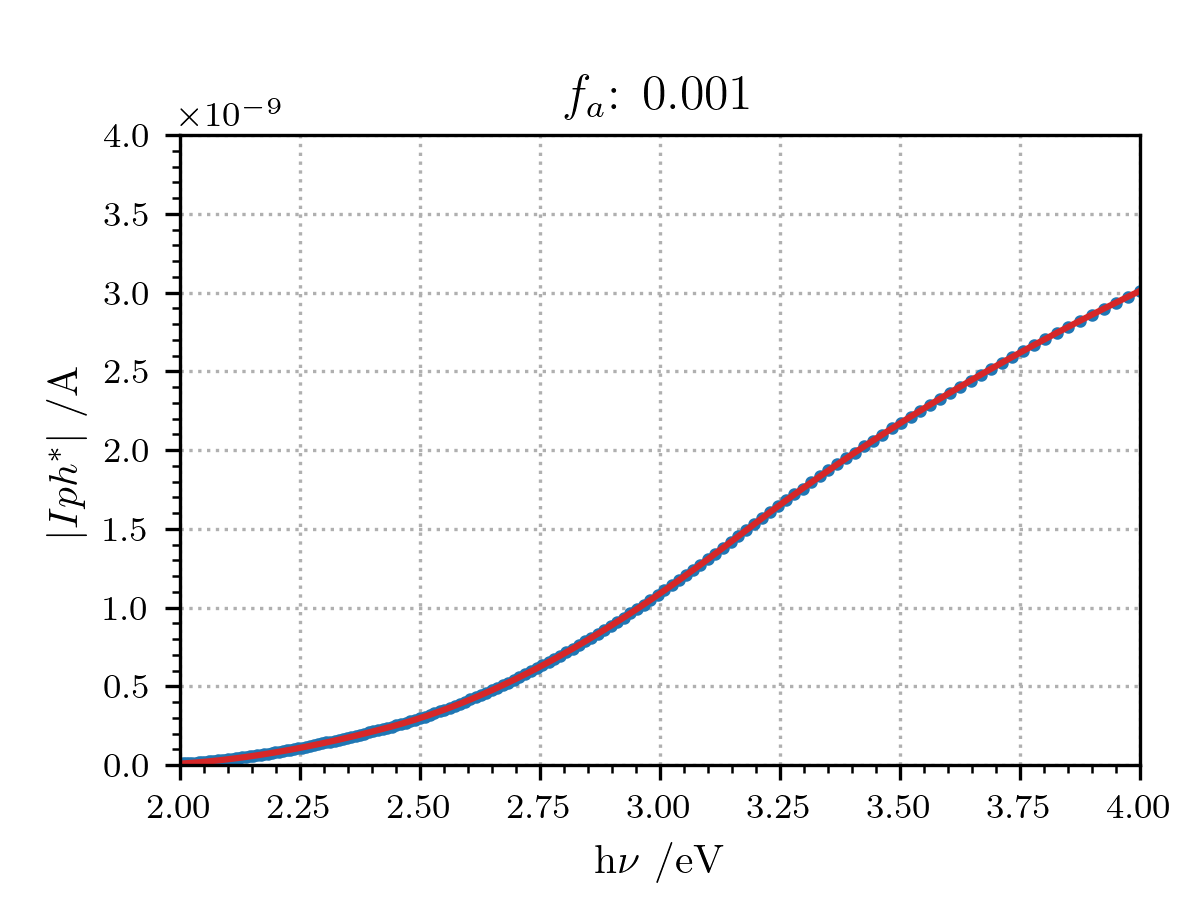
\includegraphics[width=\textwidth]{DSS_0mV_data-Iph-0001x.png}
	 	\caption{$f_a=0.001$}
	 	\label{fig:fa0001}
	\end{subfigure}
	\begin{subfigure}{\coef\textwidth}
		\centering
	 	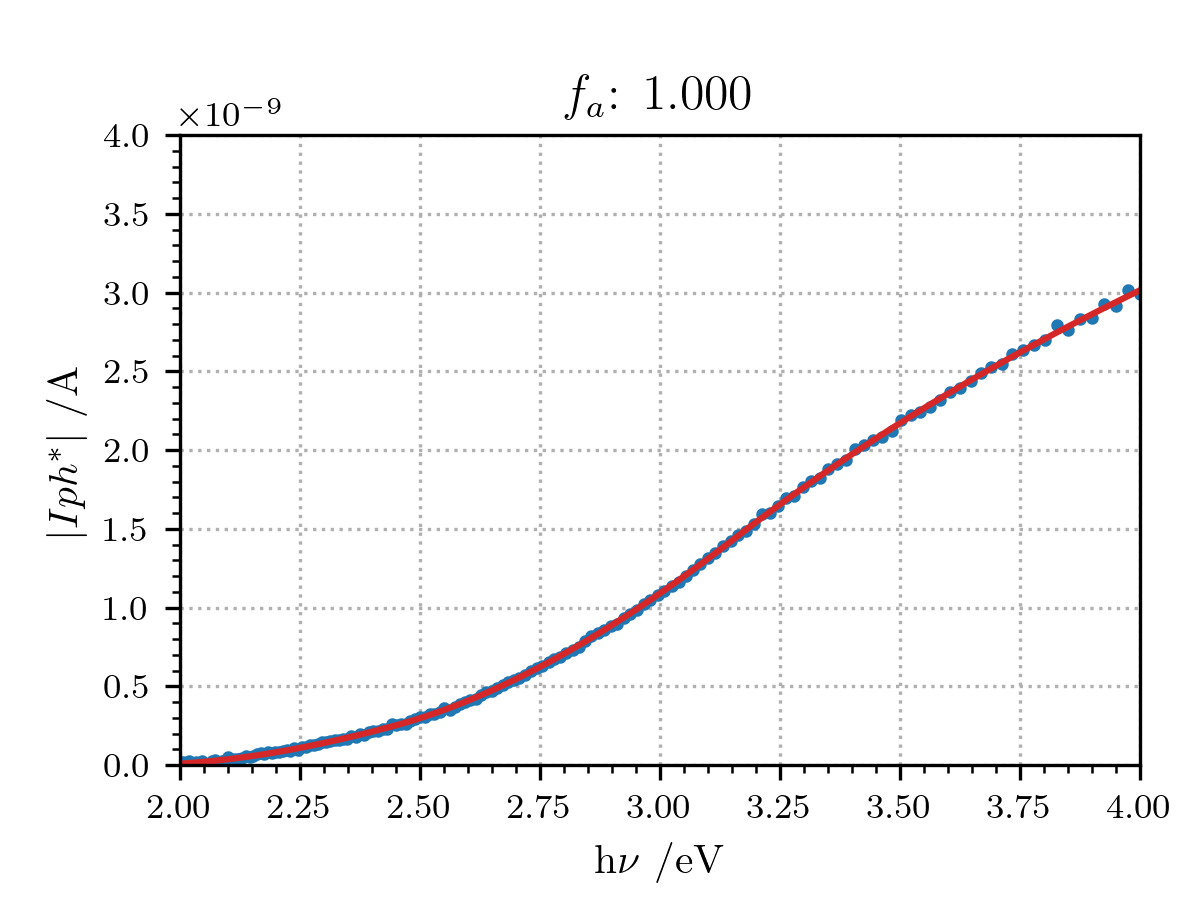
\includegraphics[width=\textwidth]{DSS_0mV_data-Iph-1x.png}
	 	\caption{$f_a=1$}
	 	\label{fig:fa1}
	\end{subfigure}
	\begin{subfigure}{\coef\textwidth}
		\centering
	 	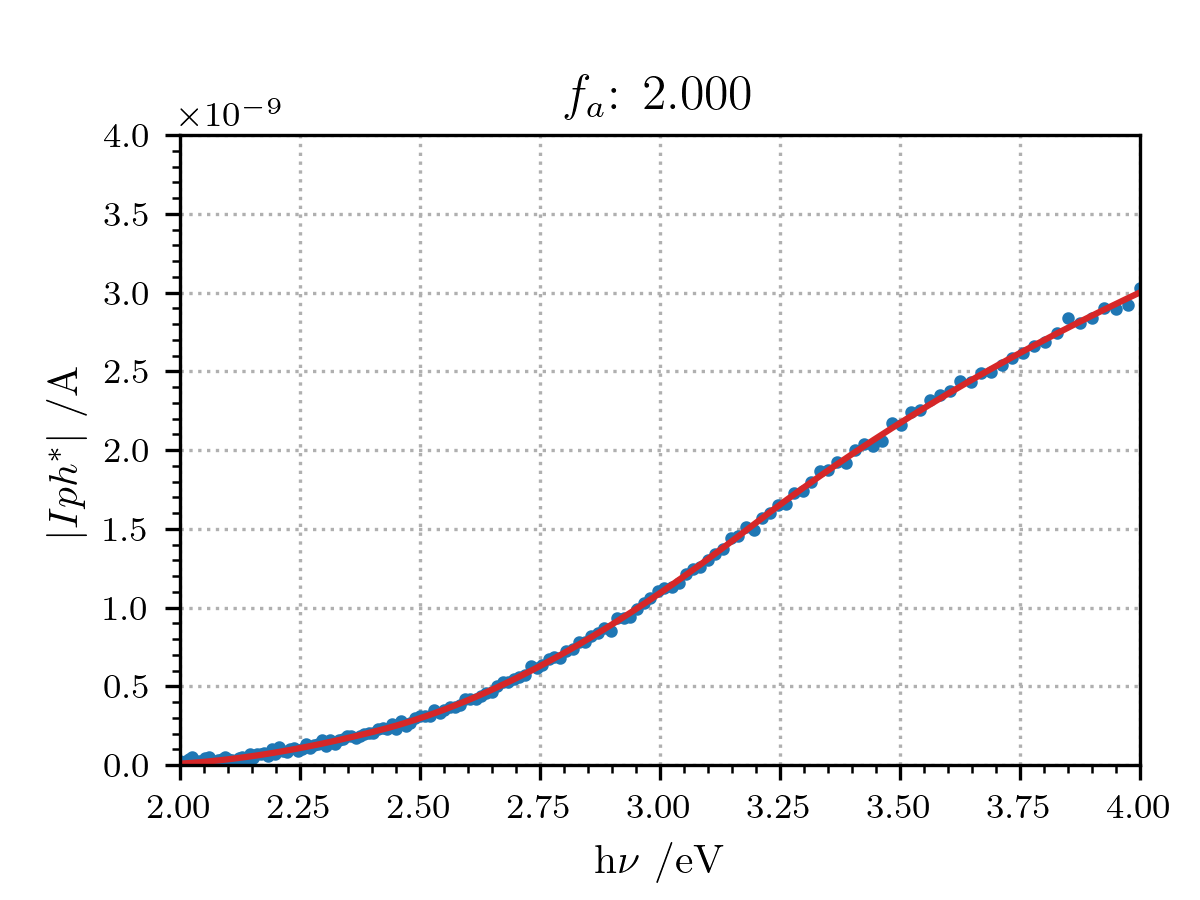
\includegraphics[width=\textwidth]{DSS_0mV_data-Iph-2x.png}
	 	\caption{$f_a=2$}
	 	\label{fig:fa2}
	\end{subfigure}
	
	\begin{subfigure}{\coef\textwidth}
		\centering
	 	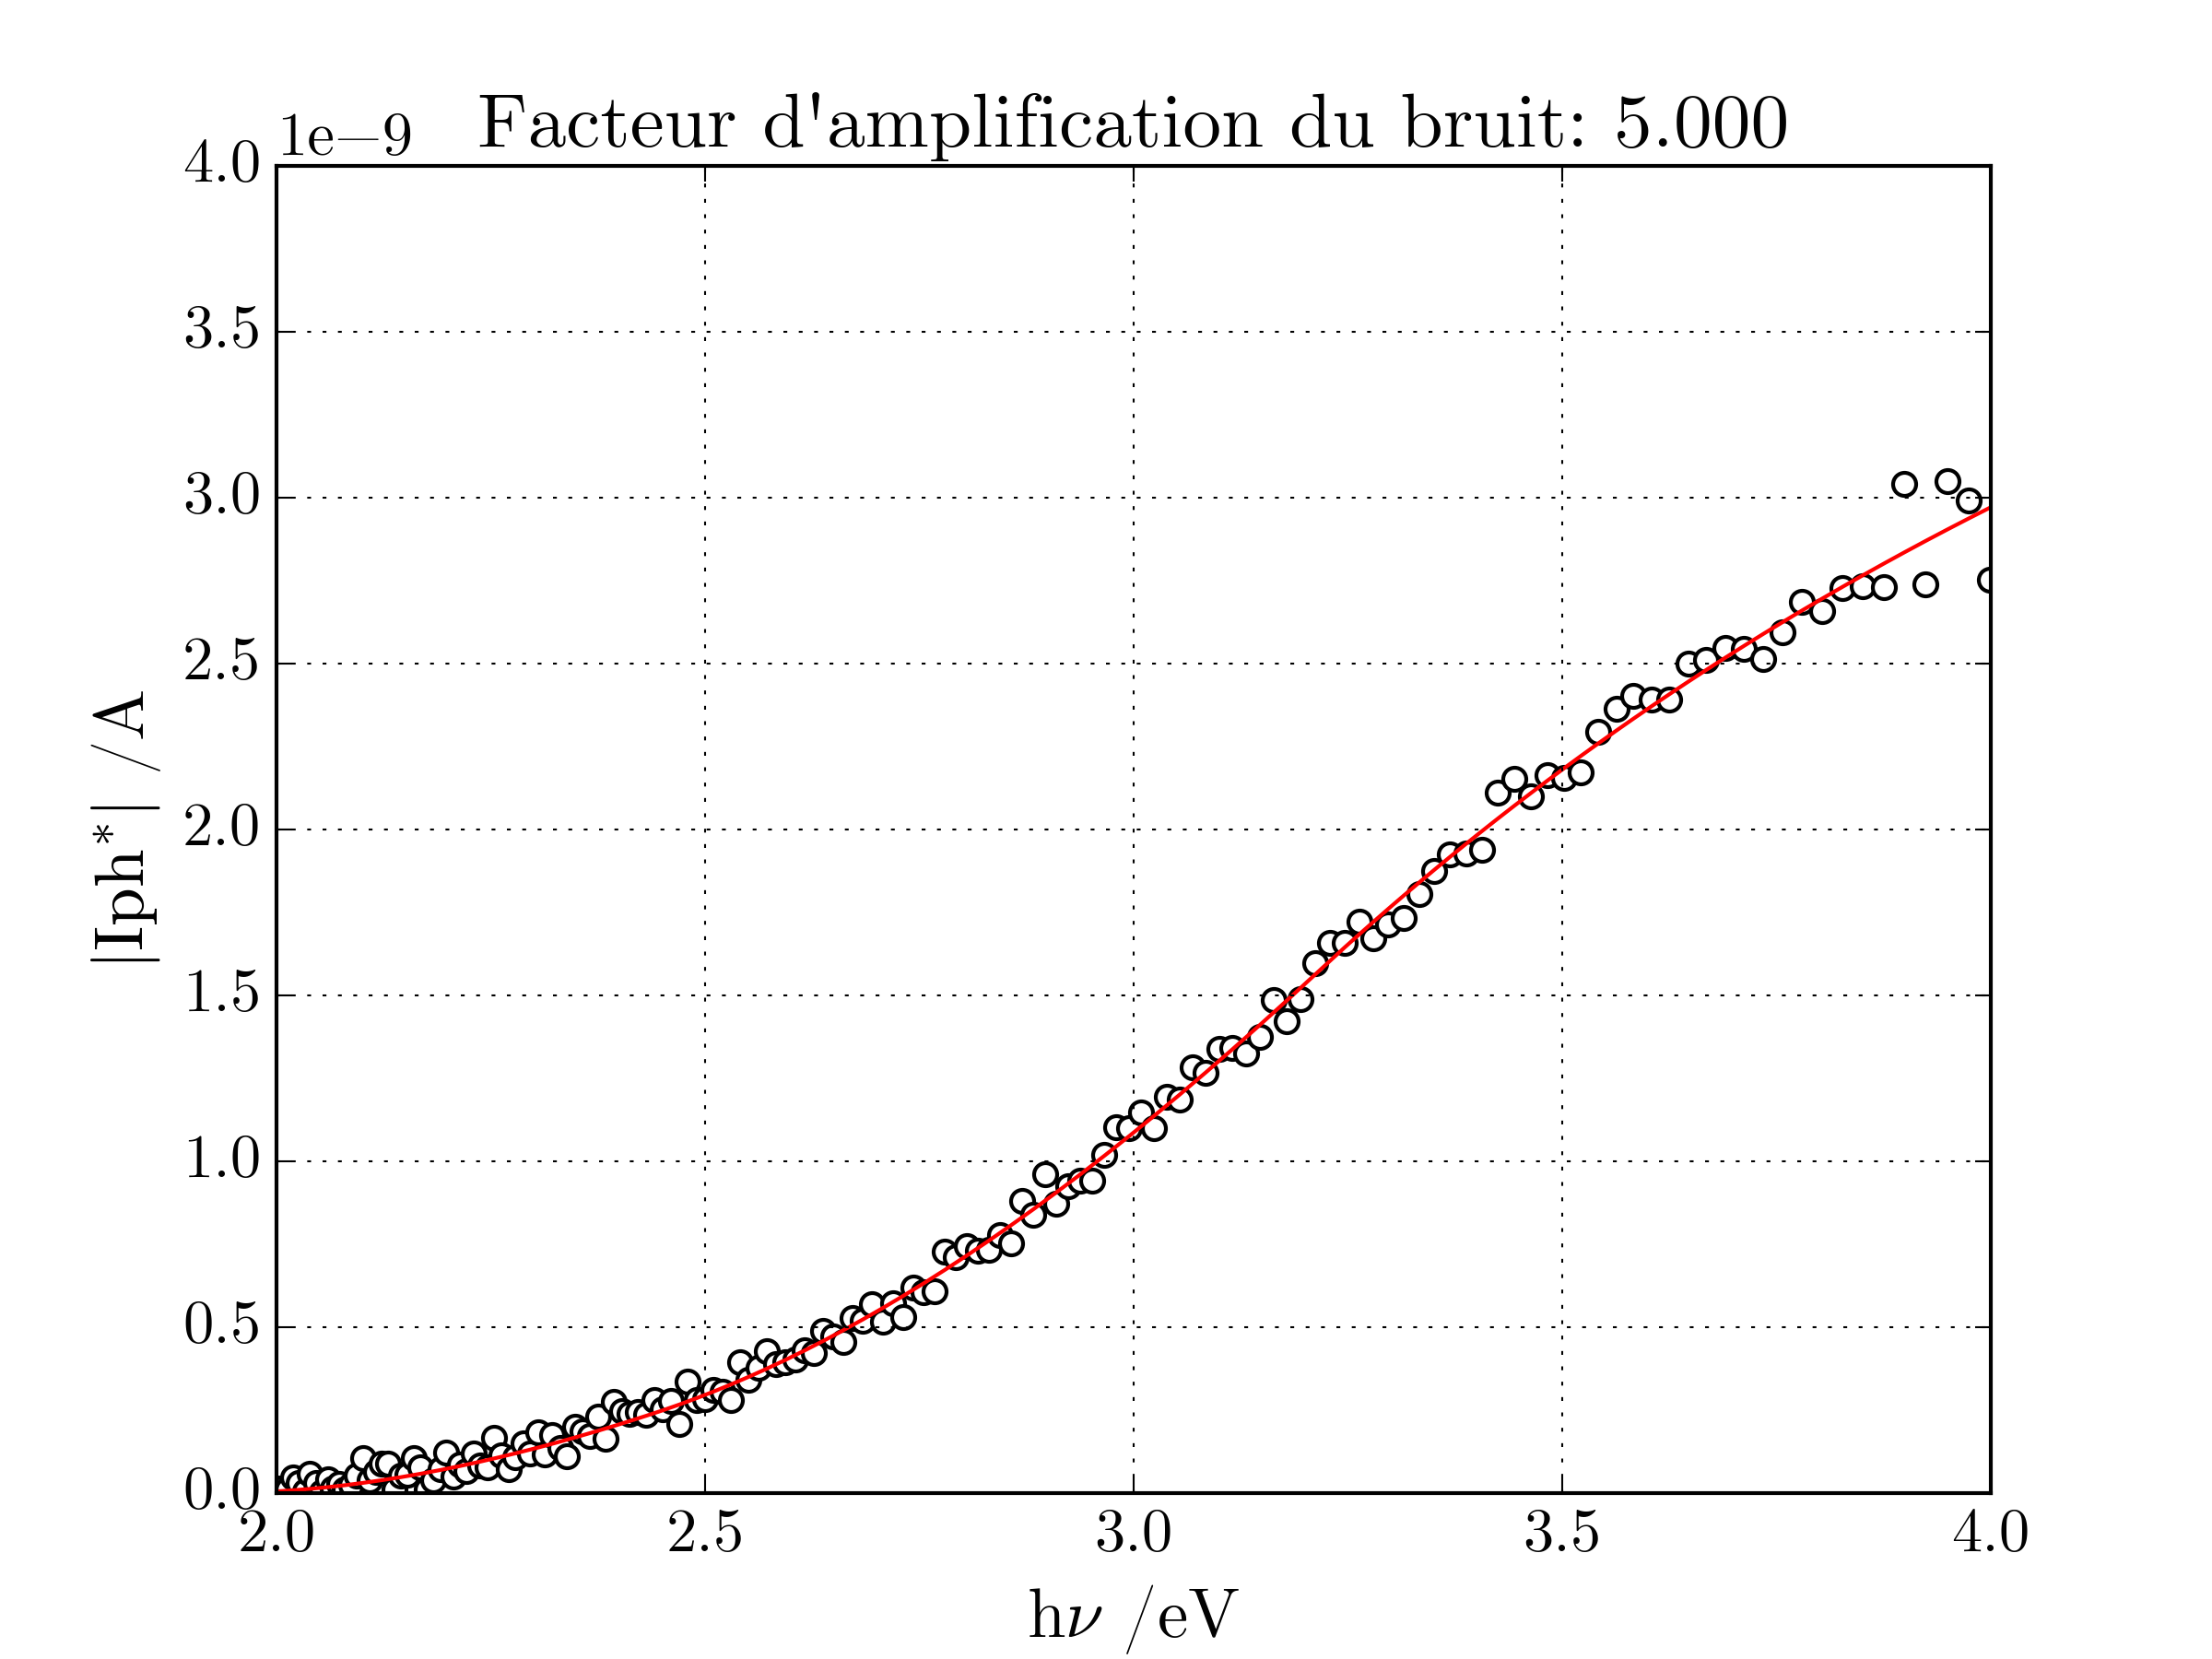
\includegraphics[width=\textwidth]{DSS_0mV_data-Iph-5x.png}
	 	\caption{$f_a=5$}
	 	\label{fig:fa5}
	\end{subfigure}\quad
	\begin{subfigure}{\coef\textwidth}
		\centering
	 	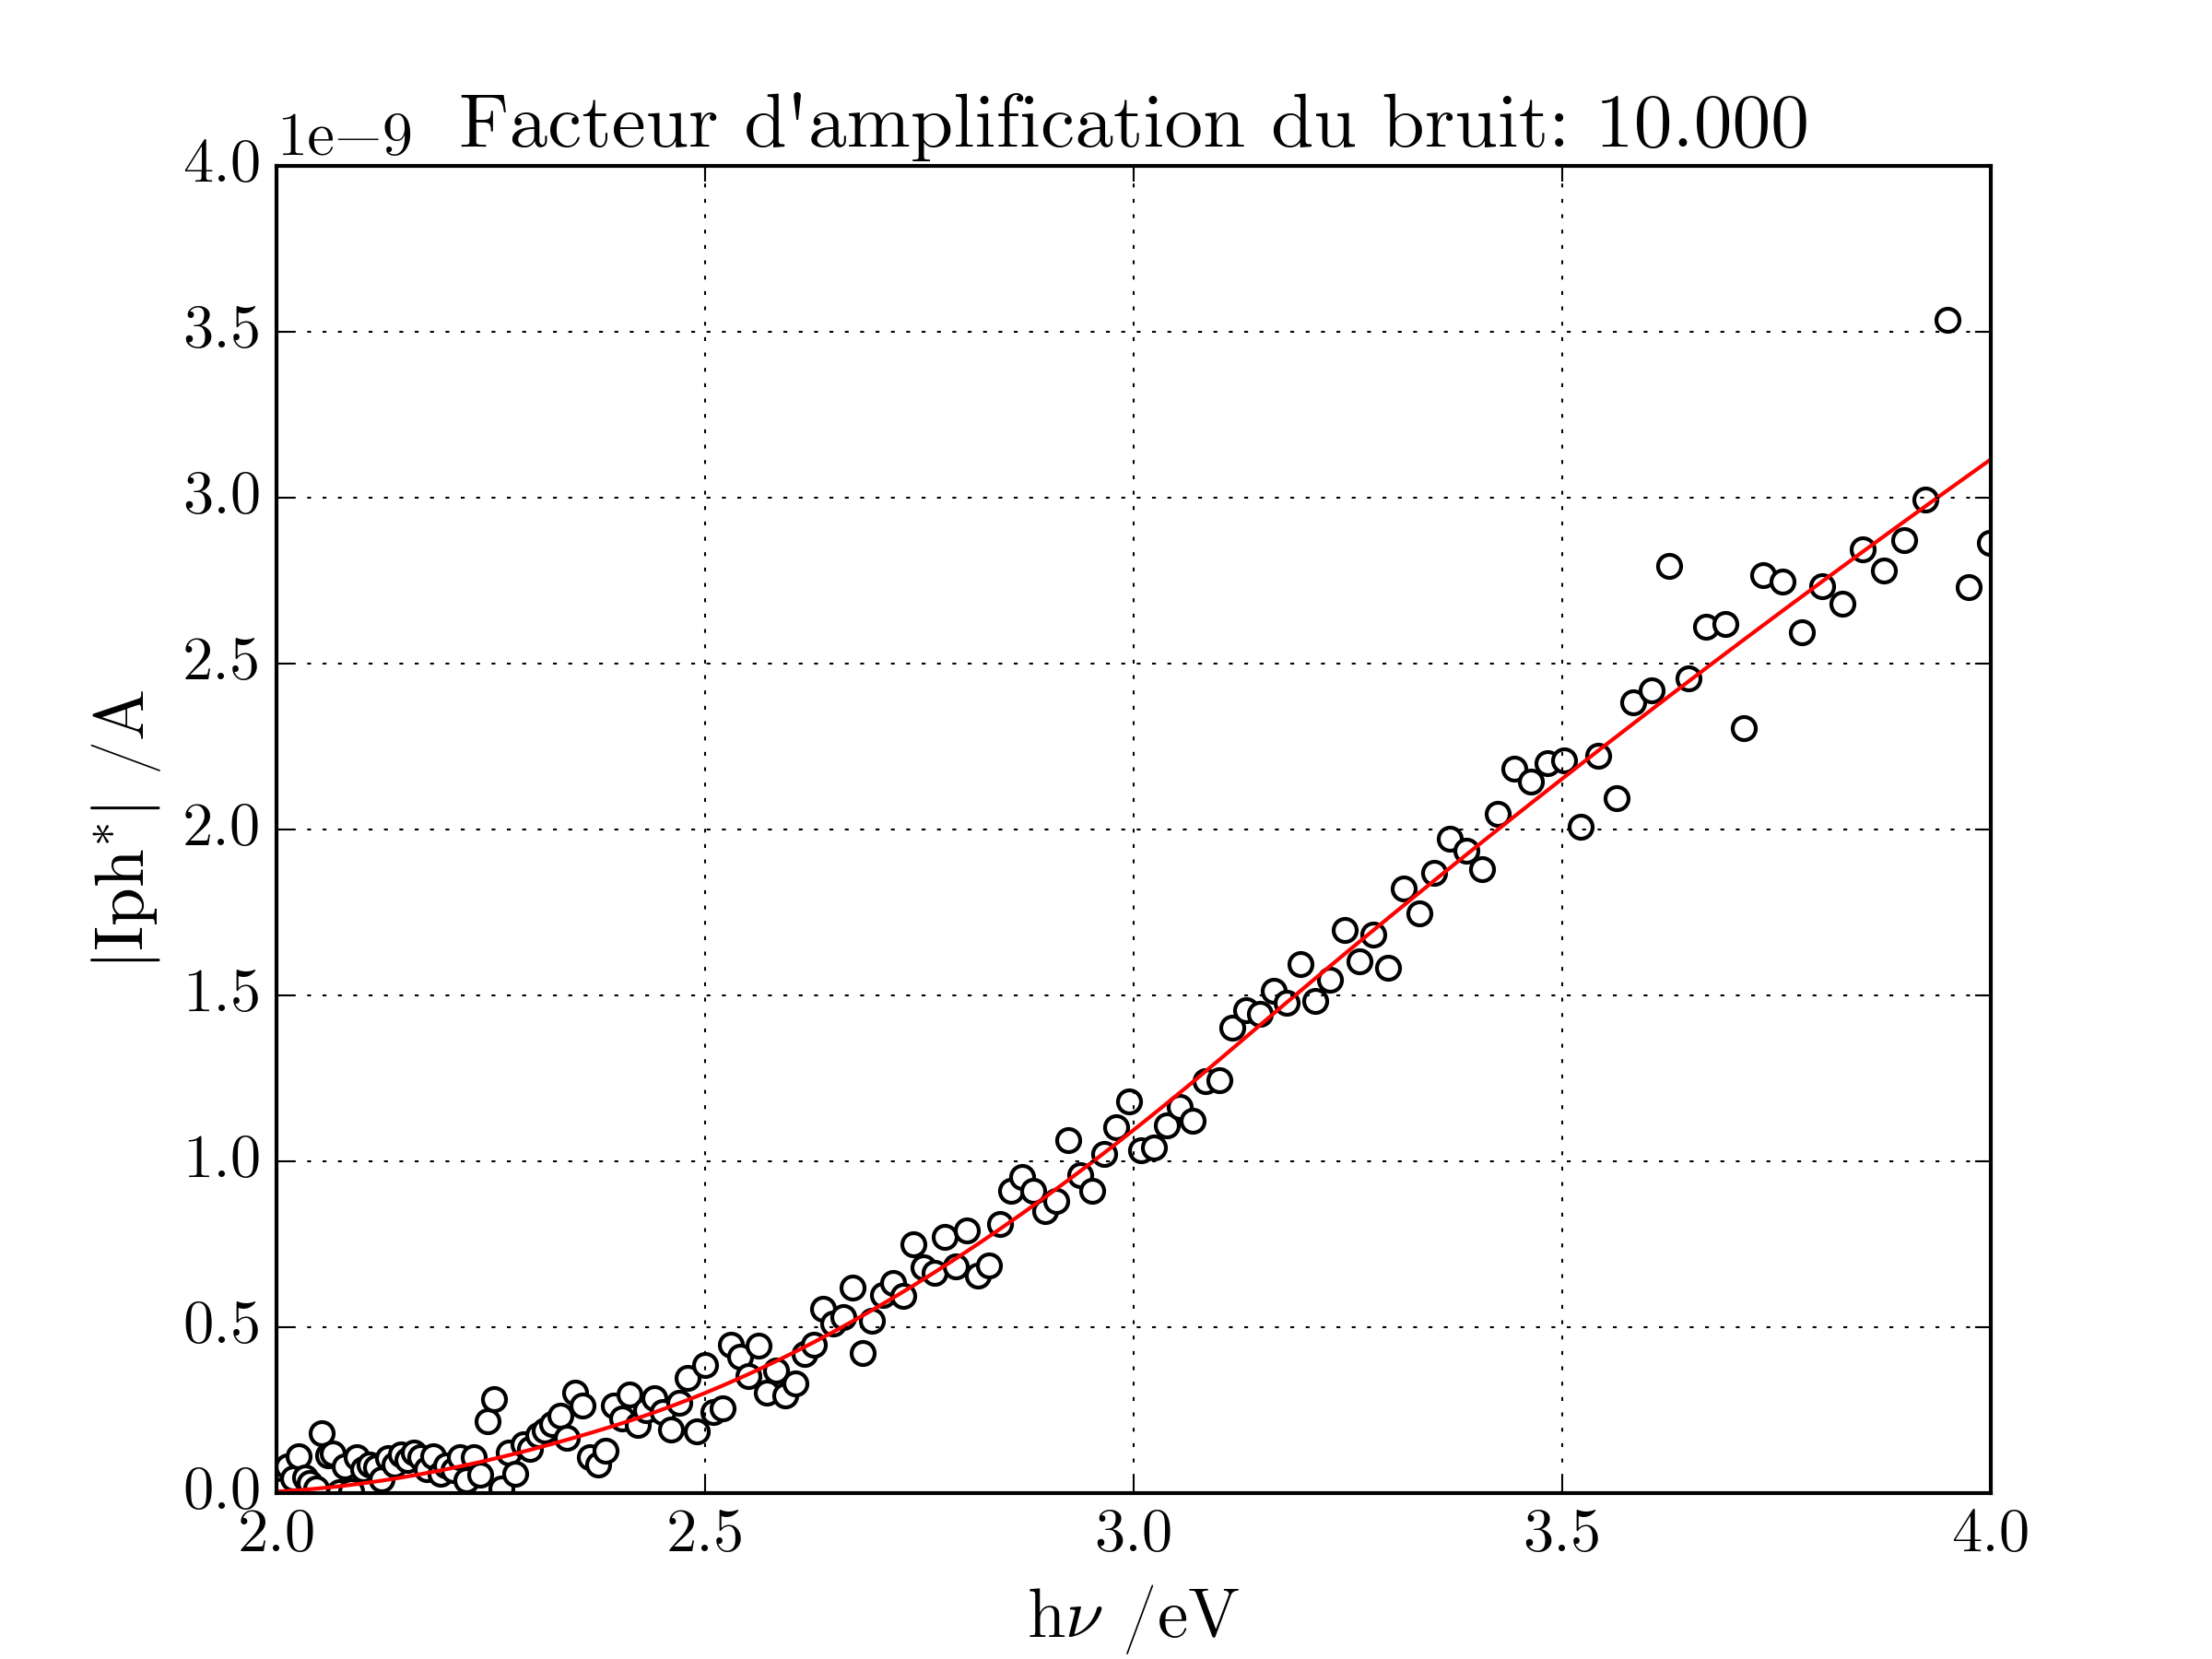
\includegraphics[width=\textwidth]{DSS_0mV_data-Iph-10x.png}
	 	\caption{$f_a=10$}
	 	\label{fig:fa10}
	\end{subfigure}
	\caption{Energy photocurrent spectra generated with different amplification factors $f_a$.}
	\label{fig:data_noise}
\end{figure*}

The estimation of the confidence intervals can also be helpful for determining 
the number of semiconductive contribution in an energy photocurrent spectrum. 
In fact, the determination of the number of semiconductive contributions is an 
iterative operation by adding contributions until the spectrum is correctly fitted. 
The estimation of the confidence intervals can be used as a break point of the 
iterative search when the intervals of two contributions are overlapping i.e. 
they are no more statistically discernable. 

For the sake of illustration, the energy photocurrent of the figure \ref{fig:fa0001} 
was fitted by considering 3, 4 and 5 semiconductive contributions for energies 
ranging from 1.8 eV to 4.0 eV. Table \ref{table:result_noise_contributions} 
shows the bandgap values and the associated confidence intervals obtained 
after numerical fitting. 

\begin{table}[htb]
\small
\centering
\begin{tabular}{ p{2cm}|p{4cm}|p{4cm}| p{4cm}}
\toprule
 $m$ & 3 & 4 &  5\\
\midrule
$E_{g,1}$ & $1.91 \pm 0.07$    & $1.9 \pm 0.4$      & $1.9 \pm 0.1$ \\
$E_{g,2}$ &  $2.4 \pm 0.2$      & $2 \pm 5$           & $2 \pm 4$\\
$E_{g,3}$ & $3.16 \pm 0.06$    & $2.5 \pm 0.4$     &  $2.5 \pm 0.2$\\
$E_{g,4}$ &                           &  $3.16 \pm 0.06$ &   $2.7 \pm 0.2$    \\
$E_{g,5}$ &                           &                         &    $3.2 \pm 0.1$     \\
 \bottomrule
\end{tabular}
\caption{Bandgap values and the associated confidence intervals obtained after 
    numerical fitting of the energy photocurrent spectra of the figure \ref{fig:fa0001}.}
\label{table:result_noise_contributions}
\end{table}




The numerical fitting, by considering 4 contributions, showed that the contribution 
with a bandgap value of 1.91 
eV was split into two contributions (1.9 eV and 2 eV). The second one featured 
a confidence interval in the same 
order of magnitude as the value itself i.e. the 4th contribution did not 
improve the fitting of the experimental 
data. 
The numerical fitting, by considering 5 contributions, showed that the same 
splitting of the contribution with a 
bandgap value of 1.91 eV. Moreover, the contribution with a bandgap value 
of 2.4 eV was split into two contributions (2.6 eV and 2.7 eV) whose confidence 
intervals were overlapping indicating that they were not statically discernable.

\subsection{Experimental energy photocurrent spectra}
The defined procedure for estimating the interval confidences was then applied 
to energy photocurrent spectra recorded at different potentials on a Ni-based 
alloy 600 thermally oxidized. The experimental data were provided by \citet{petit2013}. 
The experimental, as well as the fitted, modules of the corrected photocurrent 
$\vert I_{ph}^* \vert$ are illustrated in figure \ref{fig:exp_iph_fit}. 

The photocurrent modulus in dark conditions, $\bar{\epsilon _d}$, was computed 
by taking the average of the photocurrent modulus for the five highest energies 
(6.19, 6.17, 6.14 and 6.08 eV) where the emission spectrum of a Xe lamp can be 
reasonably considered close to zero. The photocurrent modulus featured a strong 
decrease for energies lower than 3 eV when the potential decreased towards more 
cathodic values indicating that the ratio signal/noise decreased as well. 

Table \ref{table:exp_iph_fit} shows the parameters and the associated confidence 
intervals obtained after numerical fitting of the experimental data. 
The increase of the computed confidence intervals for the three first contributions, 
having bandgap values lower than 3 eV, mirrored correctly the decrease of the 
ratio signal/noise observed on the experimental data in figure \ref{fig:exp_iph_fit}.

\begin{figure}[htb]
\centering
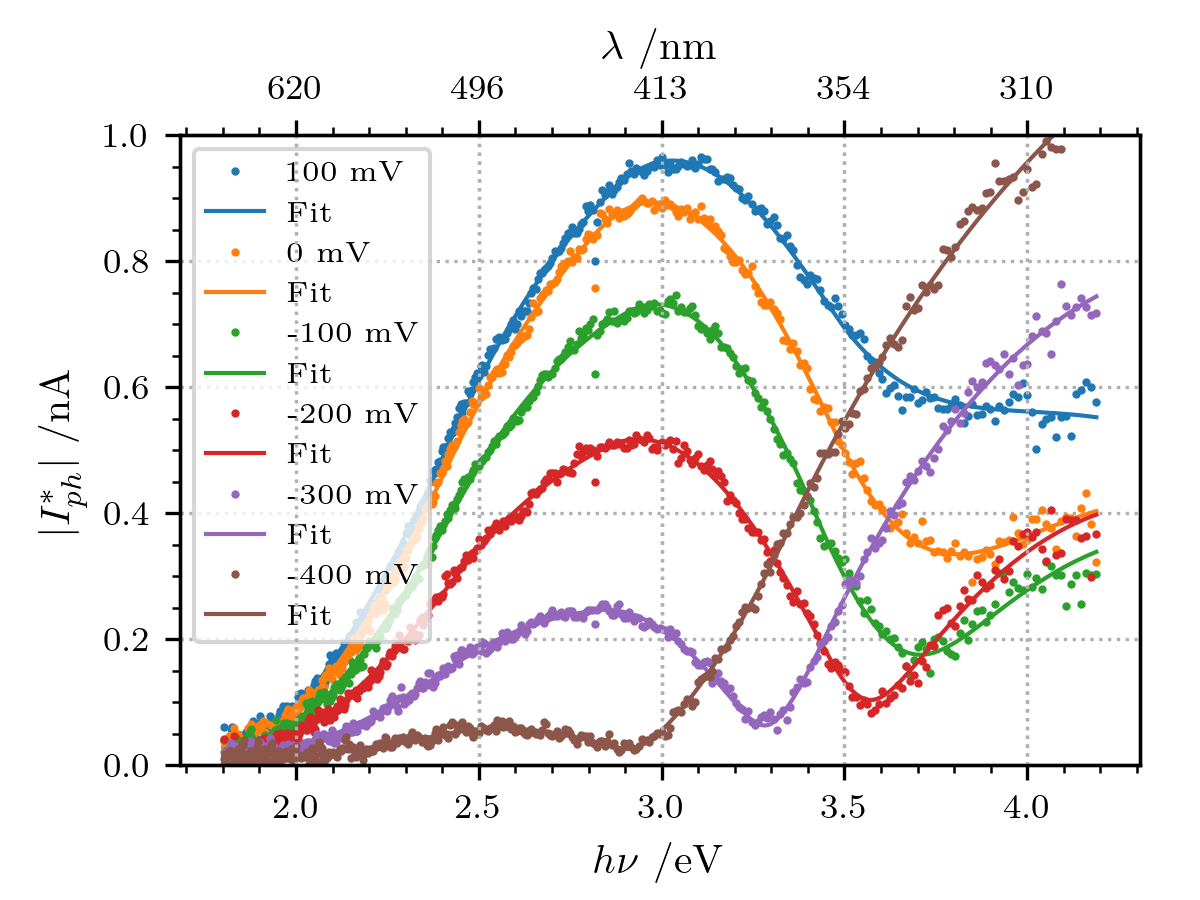
\includegraphics[width=0.65\textwidth]{Abdel-600-All-Ipht.png}
\caption{Energy photocurrent spectra recorded at different potentials on a 
    Ni-based alloy 600 thermally oxidized (experimental data were provided 
    by \citet{petit2013})}
\label{fig:exp_iph_fit}
\end{figure}

\begin{table*}[htb]
\tiny
\begin{tabular}{ p{0.5cm}|p{0.8cm}p{0.8cm}p{0.8cm}|p{0.8cm}p{0.8cm}p{0.8cm}|p{0.8cm}p{0.8cm}p{0.8cm}|p{0.8cm}p{0.8cm}p{0.8cm}}
\toprule
 $U$   & $10^5 \ K_i$ & $\theta _i$ &  $E_{g,i}$ & $10^5 \ K_i$ & $\theta _i$ &  $E_{g,i}$ & $10^5 \ K_i$ & $\theta _i$ &  $E_{g,i}$ & $10^5 \ K_i$ & $\theta _i$ &  $E_{g,i}$\\
 $mV$ & $A^{1/2} \cdot eV^{1/2}$ & ° & $eV$ & $A^{1/2} \cdot eV^{1/2}$ & ° & $eV$ & $A^{1/2} \cdot eV^{1/2}$ & ° & $eV$ & $A^{1/2} \cdot eV^{1/2}$ & ° & $eV$\\
\midrule
100   & $5.19 \pm 0.09$ & $-42.6 \pm 0.5$  & $1.74 \pm 0.02$ 
         & $6.4 \pm 0.4$ & $122 \pm 2$ & $2.42 \pm 0.04$ 
         & $6.5 \pm 0.4$ & $134 \pm 4$ & $2.88 \pm 0.05$ 
         & $8.9 \pm 0.8$ & $-64 \pm 6$ & $3.47 \pm 0.06$\\

\midrule
0   & $5.14 \pm 0.07$ & $-49.2 \pm 0.5$  & $1.755 \pm 0.008$ 
     & $6.1 \pm 0.3$ & $120 \pm 2$ & $2.41 \pm 0.04$ 
     & $6.8 \pm 0.4$ & $131 \pm 4$ & $2.82 \pm 0.04$ 
     & $9.1 \pm 0.9$ & $-58 \pm 6$ & $3.48 \pm 0.06$\\

\midrule
-100   & $4.7 \pm 0.1$ & $-52.4 \pm 0.5$  & $1.76 \pm 0.02$ 
         & $6.1 \pm 0.3$ & $119 \pm 2$ & $2.44 \pm 0.03$ 
         & $6.9 \pm 0.4$ & $131 \pm 4$ & $2.91 \pm 0.04$ 
         & $9.2 \pm 0.9$ & $-56 \pm 6$ & $3.43 \pm 0.06$\\
         
\midrule
-200   & $4.01 \pm 0.06$ & $-53.5 \pm 0.6$  & $1.76 \pm 0.02$ 
         & $5.1 \pm 0.4$ & $121 \pm 3$ & $2.43 \pm 0.04$ 
         & $6.1 \pm 0.4$ & $124 \pm 4$ & $2.85 \pm 0.04$ 
         & $8.3 \pm 0.7$ & $-63 \pm 6$ & $3.46 \pm 0.06$\\
         
\midrule
-300   & $2.9 \pm 0.3$ & $-52 \pm 2$  & $1.76 \pm 0.05$ 
         & $4.2 \pm 0.6$ & $122 \pm 5$ & $2.42 \pm 0.09$ 
         & $5.7 \pm 0.5$ & $122 \pm 4$ & $2.82 \pm 0.08$ 
         & $7.6 \pm 0.3$ & $-64 \pm 3$ & $3.43 \pm 0.06$\\
         
\midrule
-400   & $1 \pm 2$ & $-50 \pm 30$  & $1.7 \pm 0.6$ 
         & $4 \pm 3$ & $120 \pm 20$ & $2.4 \pm 0.5$ 
         & $5 \pm 2$ & $130 \pm 20$ & $2.8 \pm 0.3$ 
         & $6.7 \pm 0.7$ & $-61 \pm 6$ & $3.35 \pm 0.08$\\


\bottomrule
\end{tabular}
\caption{Parameters values and the associated confidence intervals obtained 
after numerical fitting of the energy photocurrent spectra of the figure 
\ref{fig:exp_iph_fit}. The potential is referred with respect to mercury 
sulfate electrode (MSE, +650 V vs. SHE).}
\label{table:exp_iph_fit}
\end{table*}

The fitting procedure was also applied to additional photocurrent spectra 
obtained by \citet{srisrual2013} where up to 12 contributions were found to 
be statistically discernable over 3 different potentials as illustrated in 
figure \ref{fig:data_srisrual} and table \ref{table:data_srisrual}.
Applying the adequate potential, i.e. applying the adequate band bending,
the precision on the bang gap values can be enhanced in order to better
assess the whole range of band gaps that can occur in an oxide layer.

\renewcommand{\coef}{0.4}
\begin{figure*}[htb]
	\centering
	\begin{subfigure}{\coef\textwidth}
		\centering
	 	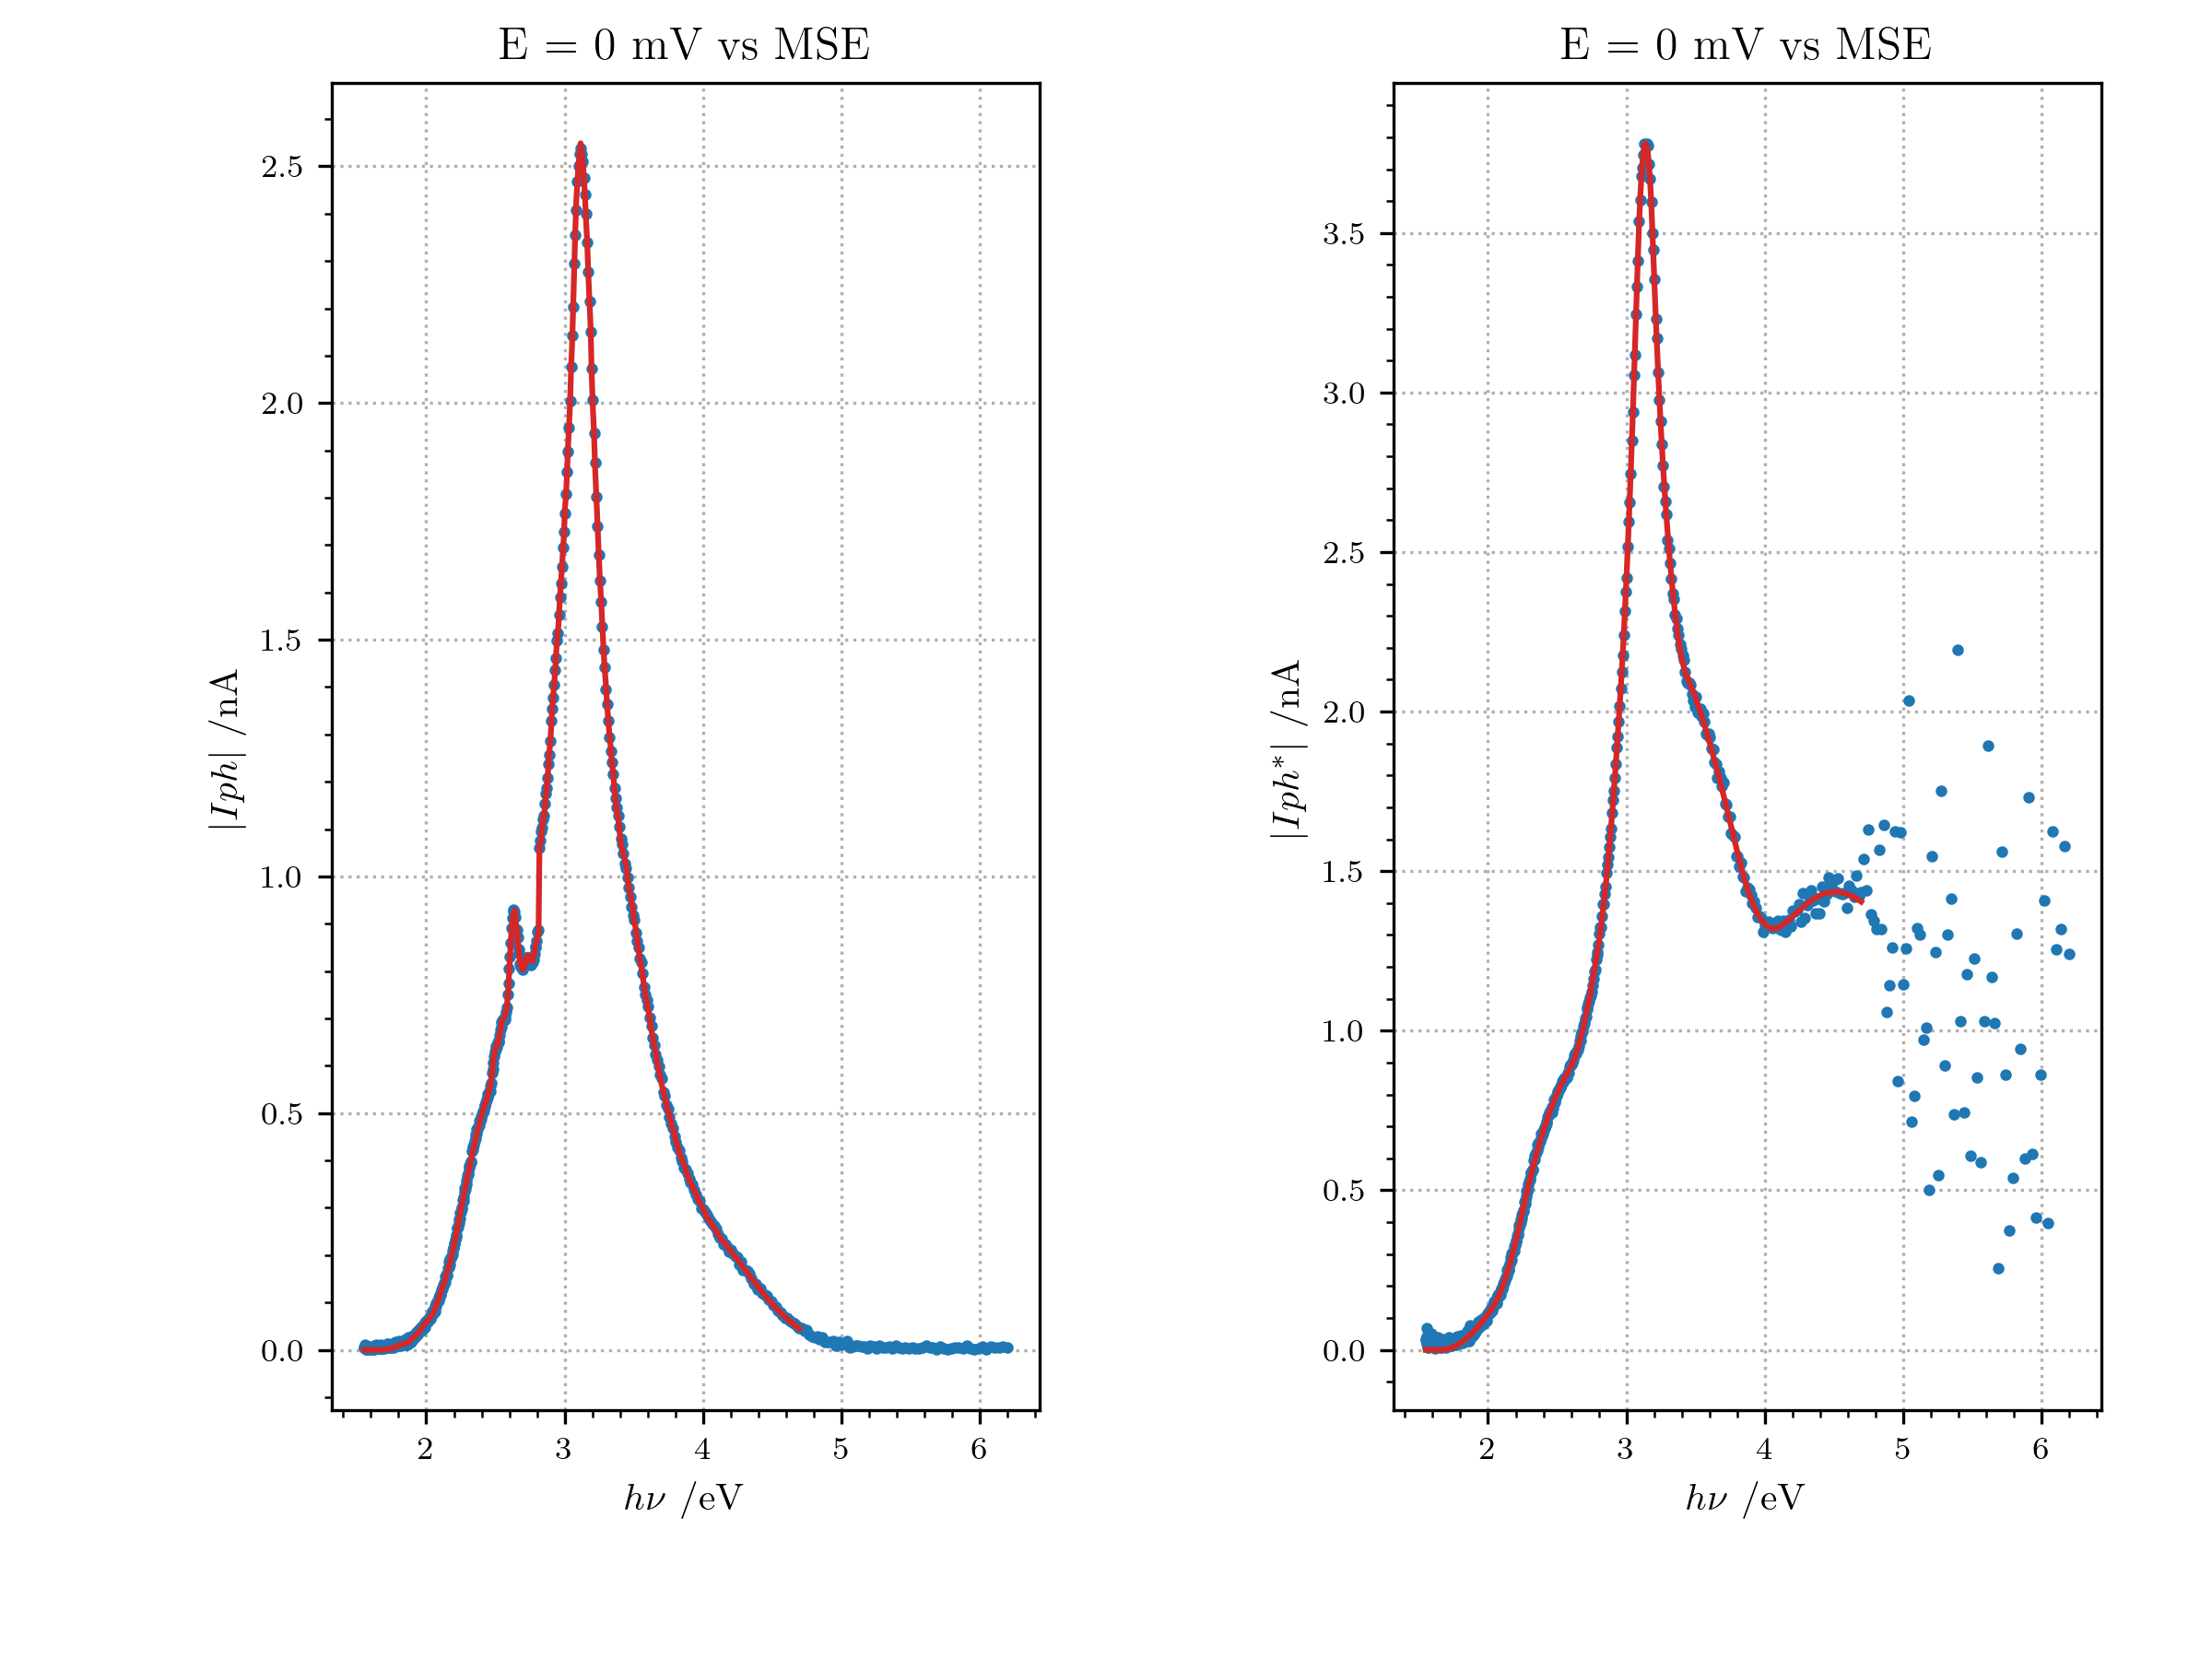
\includegraphics[width=\textwidth]{Anusara-690-0mV.png}
	 	\caption{}
	 	\label{fig:data_srisrual1}
	\end{subfigure}
	\begin{subfigure}{\coef\textwidth}
		\centering
	 	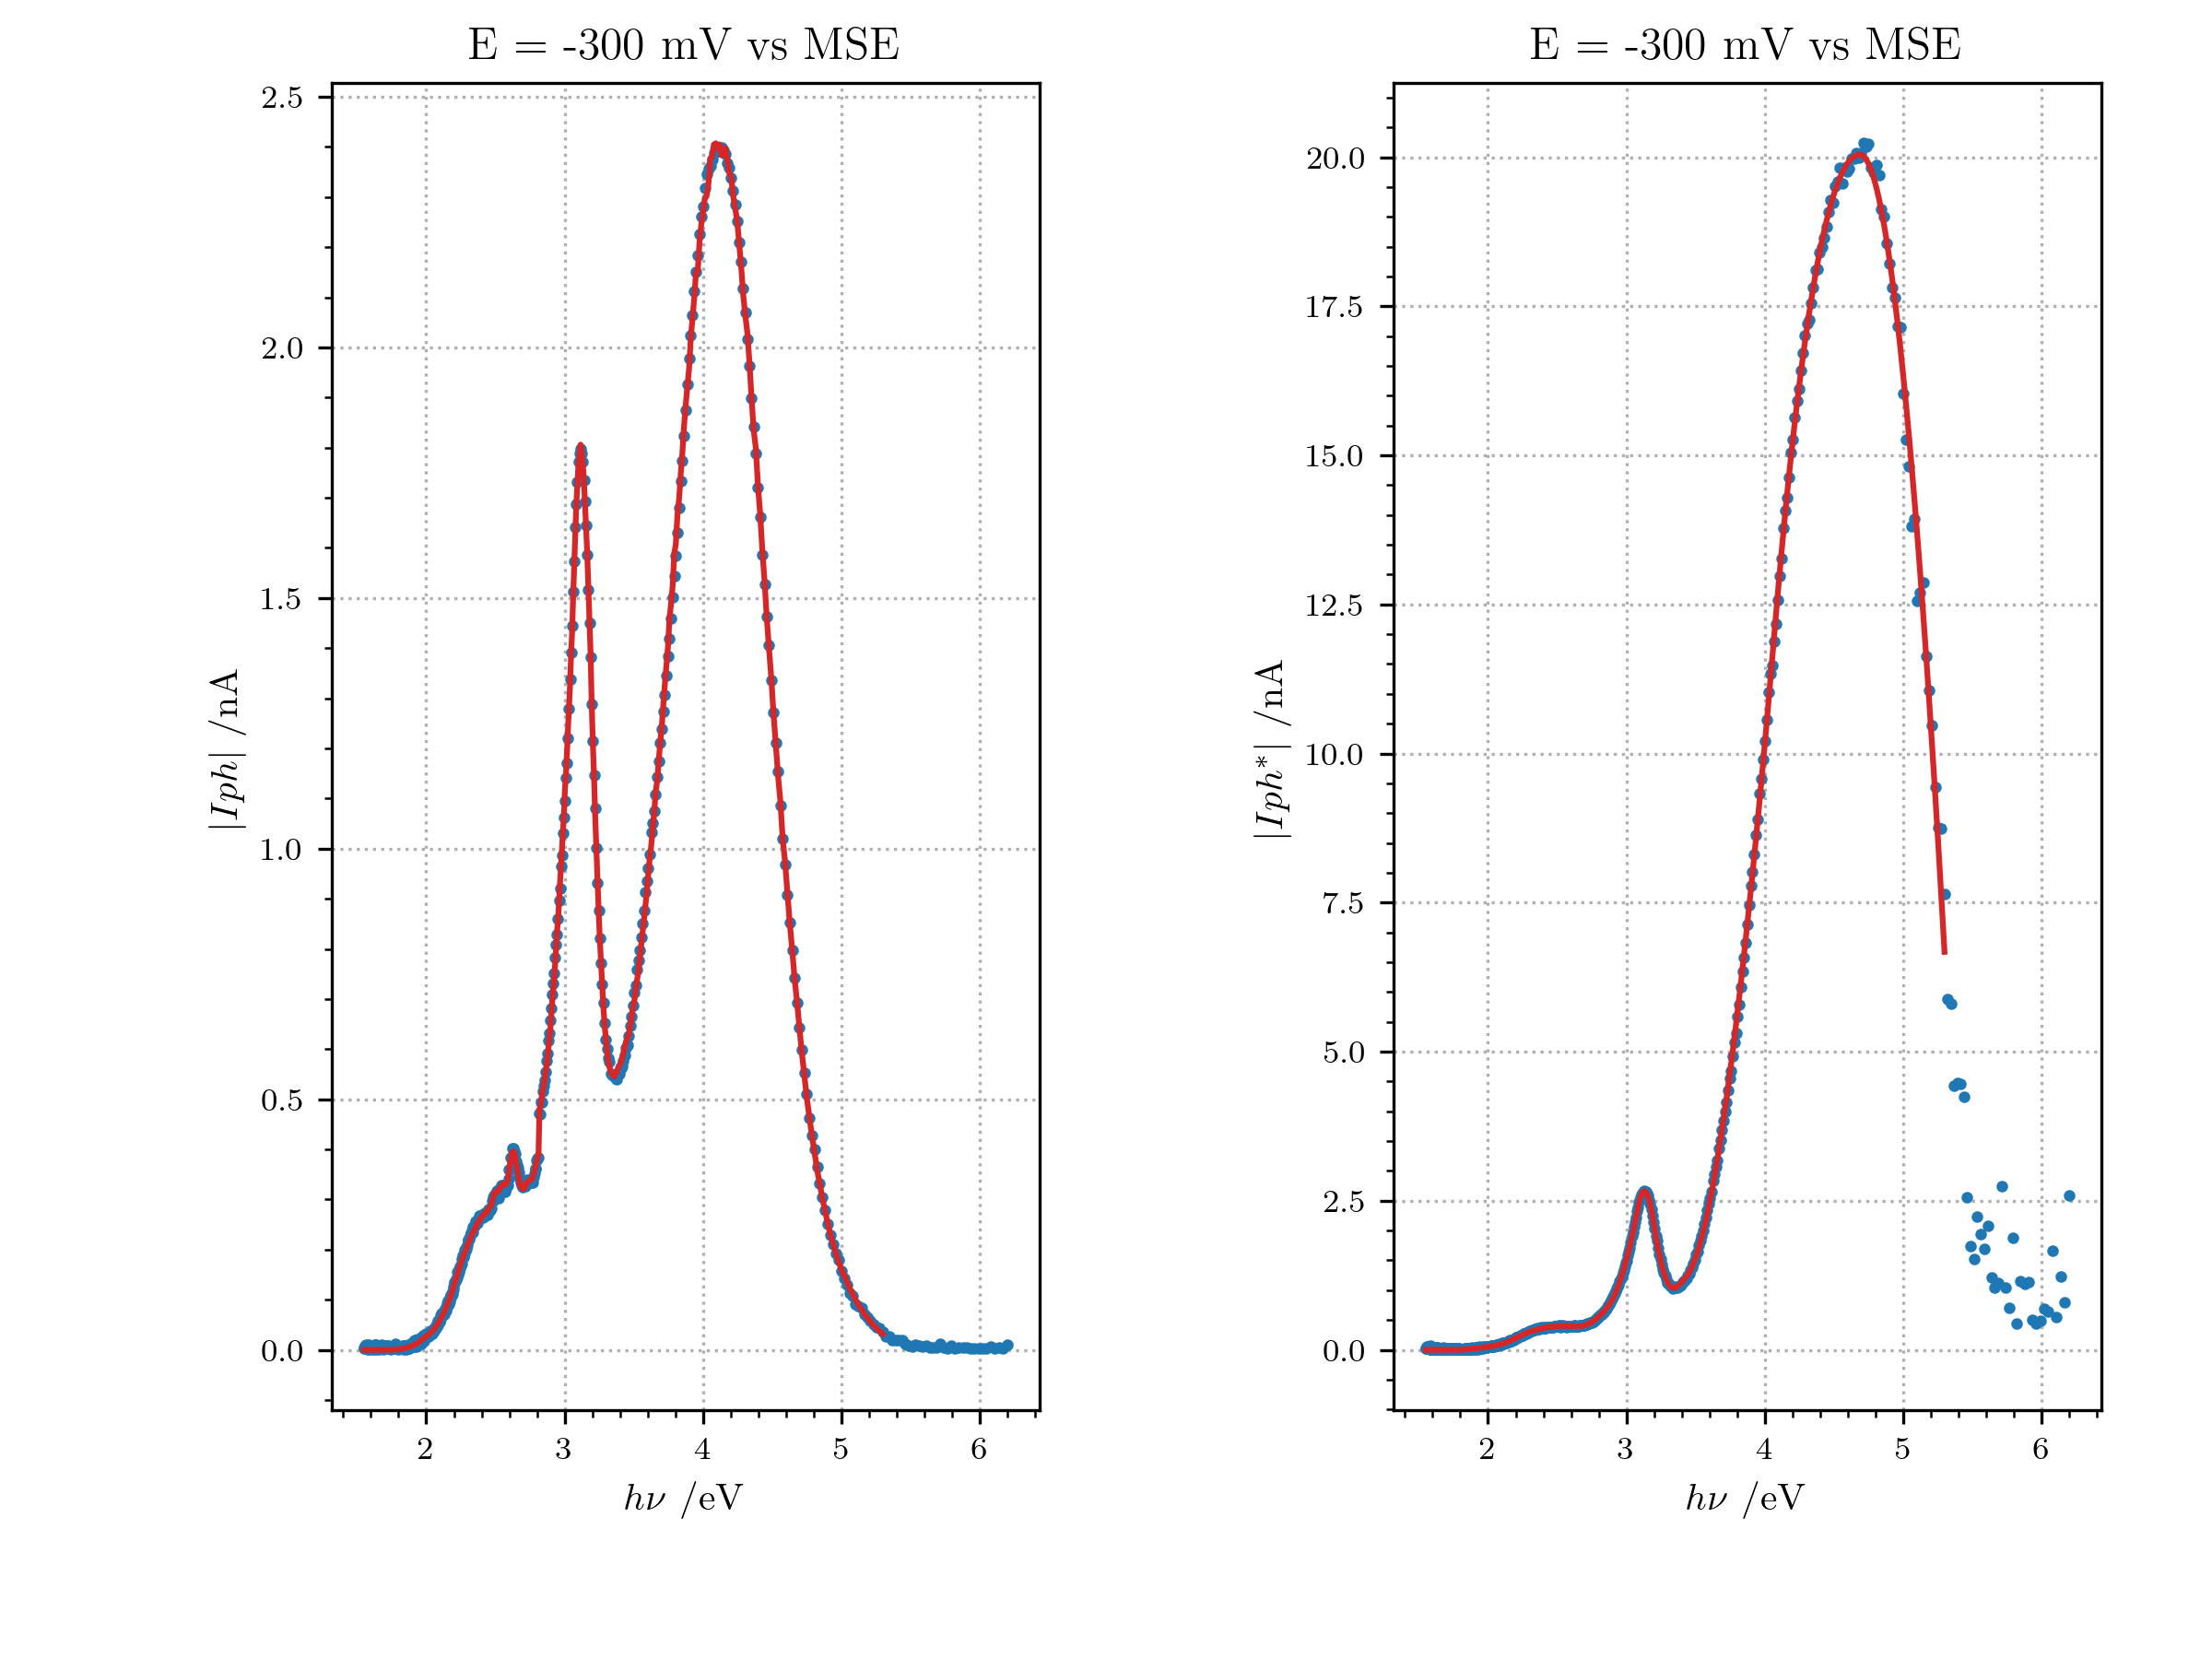
\includegraphics[width=\textwidth]{Anusara-690-300mV.png}
	 	\caption{}
	 	\label{fig:data_srisrual2}
	\end{subfigure}

	\begin{subfigure}{\coef\textwidth}
		\centering
	 	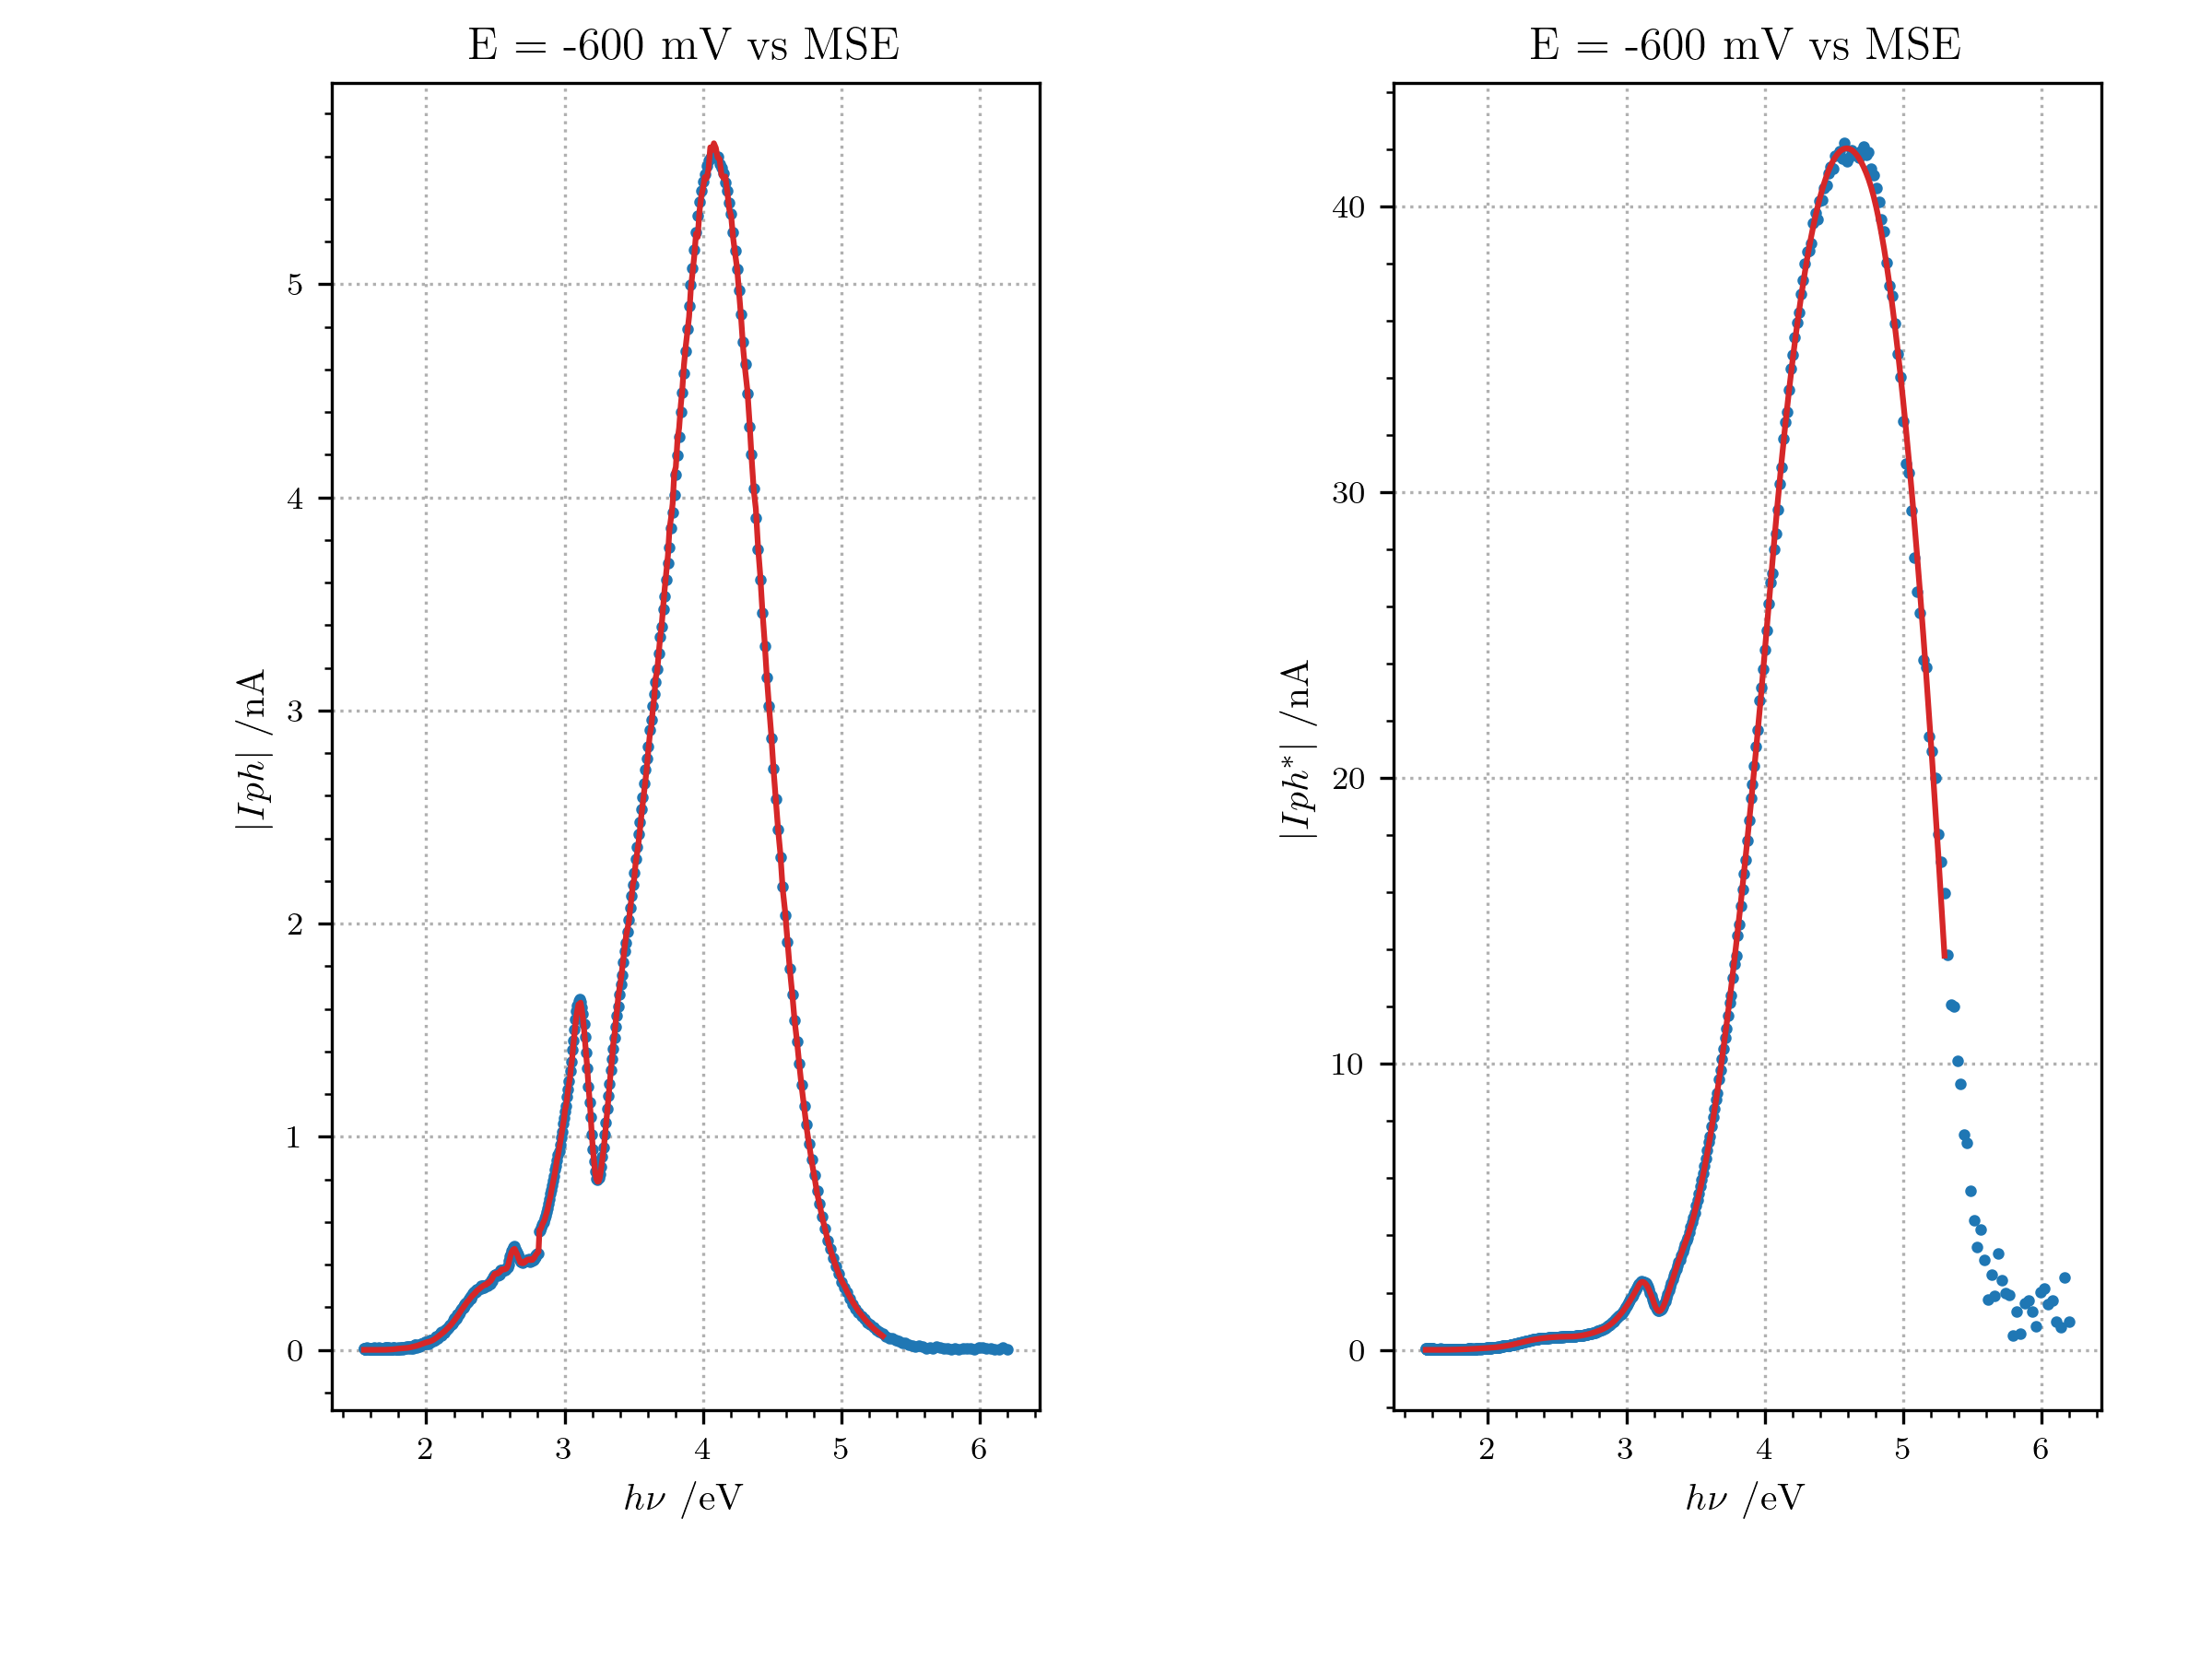
\includegraphics[width=\textwidth]{Anusara-690-600mV.png}
	 	\caption{}
	 	\label{fig:data_srisrual3}
	\end{subfigure}
	
	\caption{Energy photocurrent spectra recorded at different applied potentials 
    on a Ni-based alloy A600 oxidized at 900°C in oxygen for 2h (according to \citep{srisrual2013}).}
	\label{fig:data_srisrual}
\end{figure*}

\begin{table}[h]
\small
\centering
\begin{tabular}{ p{2cm}|p{4cm}p{4cm} p{4cm}}
\toprule
                & $0 mV_{MSE}$ & $-300 mV_{MSE}$ & $-600 mV_{MSE}$ \\
\midrule
$E_{g,1}$   & $1.7 \pm 0.2$ & $2 \pm 3$ & $2 \pm 20$ \\
$E_{g,2}$   & $2.0 \pm 0.2$ & $2 \pm 3$ & $2 \pm 8$ \\
$E_{g,3}$   & $2.25 \pm 0.09$ & $2 \pm 1$ & $2 \pm 4$ \\
$E_{g,4}$   & $2.58 \pm 0.04$ & $2.6 \pm 0.3$ & $3 \pm 2$ \\
$E_{g,5}$   & $2.8 \pm 0.04$ & $2.9 \pm 0.2$ & $2.8 \pm 0.9$ \\
$E_{g,6}$   & $2.96 \pm 0.02$ & $3.08 \pm 0.01$ & $3.09 \pm 0.05$ \\
$E_{g,7}$   & $3.077 \pm 0.0022$ & $3.16 \pm 0.03$ & $3.2 \pm 0.2$ \\
$E_{g,8}$   & $3.195 \pm 0.003$ & $3.19 \pm 0.02$ & $3.2 \pm 0.05$ \\
$E_{g,9}$   & $3.27 \pm 0.02$ & $3.42 \pm 0.03$ & $3.42 \pm 0.04$ \\
$E_{g,10}$   & $3.44 \pm 0.03$ & $4.073 \pm 0.009$ & $4.047 \pm 0.008$ \\
$E_{g,11}$   & $3.8 \pm 0.3$ & $4.7 \pm 0.1$ & $4.7 \pm 0.2$ \\
$E_{g,12}$   & $4.1 \pm 0.5$ &  &  \\
     
\bottomrule
\end{tabular}
\caption{Parameters values and the associated confidence intervals obtained 
    after numerical fitting of the energy photocurrent spectra of the figure \ref{fig:data_srisrual}}
\label{table:data_srisrual}
\end{table}

\section{Conclusion} 

The weighting terms for the numerical fitting procedure were defined using 
the definition of the $\chi ^2$ distribution and a scaling factor for the covariance matrix.
The latter correctly reflected the noise of the experimental data in the computed 
i.e. the covariance matrix will correctly estimate the confidence intervals 
for the fitted parameters. 

Moreover, the confidence intervals were helpful for determining the number of 
semiconductive contributions. The estimation of the confidence intervals can 
be used as a break point of the iterative search when the intervals of two 
contributions are overlapping i.e. they are no more statistically discernable. 

Experimental spectra were tested with up to 12 contributions over 3 different 
potentials and the estimated confidence intervals were helpfull at asserting 
that the semiconductive contributions are statistically discernable.





\backmatter
\pagestyle{plain}

\end{document}

